\documentclass[tikz,margin=1cm]{standalone}

\usepackage{bm}

\makeatletter
\def\mathcolor#1#{\@mathcolor{#1}}
\def\@mathcolor#1#2#3{%
	\protect\leavevmode
	\begingroup\color#1{#2}#3\endgroup
}
\makeatother

\newcommand\differentialindex[1]{{\hspace{-0.1ex}\scalebox{0.63}{$\mathcolor{black!70}{\partial}$} #1}}

\newcommand\locationvector{\bm{r}}

\usepackage{tikz}
\usetikzlibrary{calc}
\usetikzlibrary{arrows, arrows.meta}
\usetikzlibrary{decorations.markings}
\usetikzlibrary{decorations.pathreplacing}

\begin{document}

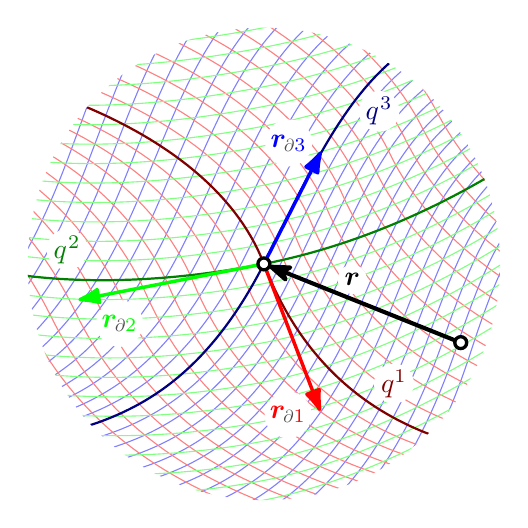
\begin{tikzpicture}[scale=0.5]

%%\clip (-6, -6) rectangle + (12, 12) ; % crop it
\clip (0, 0) circle (6cm) ; % crop it

\tikzset{%
	tangent/.style={
		decoration={
			markings,% switch on markings
			mark=
			at position #1
			with
			{
				\def\numberoftangent{\pgfkeysvalueof{/pgf/decoration/mark info/sequence number}}
				\coordinate (tangent point-\numberoftangent) at (0, 0);
				\coordinate (tangent unit vector-\numberoftangent) at (1, 0);
				\coordinate (tangent orthogonal unit vector-\numberoftangent) at (0, 1);
			}
		},
		postaction=decorate
	},
	use tangent/.style={
		shift=(tangent point-#1),
		x=(tangent unit vector-#1),
		y=(tangent orthogonal unit vector-#1)
	},
	use tangent/.default=1
}

\tikzset{%
	show curve controls/.style={
		postaction={
			decoration={
				show path construction,
				curveto code={
					\fill [black, opacity=.5]
						(\tikzinputsegmentfirst) circle (.4ex)
						(\tikzinputsegmentlast) circle (.4ex) ;
					\draw [black, opacity=.5, line cap=round, dash pattern=on 0pt off 1.6\pgflinewidth]
						(\tikzinputsegmentfirst) -- (\tikzinputsegmentsupporta)
						(\tikzinputsegmentlast) -- (\tikzinputsegmentsupportb) ;
					\fill [magenta, opacity=.5, line cap=round, dash pattern=on 0pt off 1.6\pgflinewidth]
						(\tikzinputsegmentsupporta) circle [radius=.4ex]
						(\tikzinputsegmentsupportb) circle [radius=.4ex] ;
				}
			},
			decorate
}	}	}

%%\foreach \cycle in {0, 1, ..., 15}
%%	\draw [color=green]
%%		($ (0, 0) - (\cycle, 1.2*\cycle) $)
%%		parabola ($ (4, 3) + 0.5*(1.6*\cycle, \cycle) $);

\foreach \c in {-10, -9.5, ..., 10}
{
	\def\offset{0.2*\c, -0.1*\c}
	\pgfmathsetmacro\bottomoffsetx{-.24 * ( \c )}
	\pgfmathsetmacro\bottomoffsety{-.1 * abs( \c ) + .1 * ( \c )}
	\pgfmathsetmacro\bottomangle{12 - 1.2 * abs( \c )}
	\pgfmathsetmacro\bottomnudge{2}
	\pgfmathsetmacro\midoffsetx{-.1 * abs( \c )}
	\pgfmathsetmacro\midoffsety{.1 * abs( \c )}
	\pgfmathsetmacro\midangle{63 + 1.2 * abs( \c )}
	\pgfmathsetmacro\midnudge{4 + ( .1 * abs( \c ) )}
	\pgfmathsetmacro\topoffsetx{.32 * ( \c ) + 0 * abs( \c )}
	\pgfmathsetmacro\topoffsety{-.16 * ( \c ) + 0 * abs( \c )}
	\pgfmathsetmacro\topangle{166 + 1.6 * ( \c ) + 1.2 * abs( \c )}
	\pgfmathsetmacro\topnudge{5 + ( .25 * abs( \c ) )}
	\draw	[ line width=.4pt
		, color=blue!50
		%%, show curve controls
		]
		($ (-6, -4.5) + 5*(\offset) + (\bottomoffsetx, \bottomoffsety) $)
		.. controls ++(\bottomangle: \bottomnudge) and ++(\midangle: -\midnudge) ..
		($ 4*(\offset) + (\midoffsetx, \midoffsety) $)
		.. controls ++(\midangle: \midnudge) and ++(\topangle: \topnudge) ..
		($ (8, 6) + 2.5*(\offset) + (\topoffsetx, \topoffsety) $) ;
}

\foreach \c in {-10, -9.5, ..., 10}
{
	\def\offset{0.2*\c, 0.1*\c}
	\pgfmathsetmacro\leftoffsetx{- .1 * abs ( \c )}
	\pgfmathsetmacro\leftoffsety{.4 * ( \c )}
	\pgfmathsetmacro\leftangle{33 + .2 * abs( \c )}
	\pgfmathsetmacro\leftnudge{1.6 + .5 * abs( \c )}
	\pgfmathsetmacro\midoffsetx{-.2 * abs( \c )}
	\pgfmathsetmacro\midoffsety{.2 * abs( \c )}
	\pgfmathsetmacro\midangle{111 + 1.2 * abs( \c )}
	\pgfmathsetmacro\midnudge{5}
	\pgfmathsetmacro\rightoffsetx{.25 * abs( \c )}
	\pgfmathsetmacro\rightoffsety{.16 * ( \c )}
	\pgfmathsetmacro\rightangle{177 + 2 * ( \c )}
	\pgfmathsetmacro\rightnudge{abs( 2 - ( .5 * ( \c ) ) )}
	\draw	[ line width=.4pt
		, color=red!50
		%%, show curve controls
		]
		($ (-12, 5) + 2.5*(\offset) + (\leftoffsetx, \leftoffsety) $)
		.. controls ++(\leftangle: \leftnudge) and ++(\midangle: \midnudge) ..
		($ 5*(\offset) + (\midoffsetx, \midoffsety) $)
		.. controls ++(\midangle: -\midnudge) and ++(\rightangle: \rightnudge) ..
		($ (8, -5) + 4*(\offset) + (\rightoffsetx, \rightoffsety) $);
}

\foreach \c in {-10, -9.5, ..., 10}
{
	\def\offset{0*\c, 0.25*\c}
	\pgfmathsetmacro\midnudge{6 + .16 * ( \c )}
	\draw	[ line width=.4pt
		, color=green!50
		%%, show curve controls
		]
		($ (12, 10) + 4*(\offset) $)
		.. controls ++(88: -4) and ++(11: \midnudge) ..
		($ 4*(\offset) $)
		.. controls ++(11: -\midnudge) and ++(99: -4) ..
		($ (-12, 4) + 4*(\offset) $) ;
}

\draw	[ line width=.8pt
	, color=blue!50!black
	%%, show curve controls
	]
	(-6, -4.5)
	.. controls ++(12: 2) and ++(63: -4) ..
	(0, 0);

\draw	[ line width=.8pt
	, color=blue!50!black
	%%, show curve controls
	, tangent=0
	, tangent=0.4
	]
	(0, 0)
	.. controls ++(63: 4) and ++(166: 5) ..
	(8, 6) ;

\path [use tangent=1]
	(0, 0) -- (.4*4, 0)
	node [color=blue, pos=0.86, above left, shape=circle, fill=white, outer sep=4pt, inner sep=1pt]
		{$\locationvector_\differentialindex{3}$} ;

\draw [line width=1.25pt, color=blue, use tangent=1, -{Latex[round, length=3.6mm, width=2.4mm]}]
	(0, 0) -- (.4*4, 0) ;

\path [use tangent=2]
	(0, 0) -- (0, -1)
	node [color=blue!50!black, pos=0.48, above, shape=circle, fill=white, outer sep=0pt, inner sep=0.25pt]
		{$q^{\hspace{.1ex}3}$} ;

%%\fill [fill=blue, use tangent=1] (0, 0) circle (1mm);

\draw	[ line width=.8pt
	, color=red!50!black
	%%, show curve controls
	]
	(-12, 5)
	.. controls ++(33: 1.6) and ++(111: 5) ..
	(0, 0);

\draw	[ line width=.8pt
	, color=red!50!black
	%%, show curve controls
	, tangent=0
	, tangent=0.5
	]
	(0, 0)
	.. controls ++(111: -5) and ++(177: 2) ..
	(8, -5) ;

\path [use tangent=1]
	(0, 0) -- (.4*5, 0)
	node [color=red, pos=0.86, below left, shape=circle, fill=white, outer sep=4pt, inner sep=1pt]
		{$\locationvector_\differentialindex{1}$} ;

\draw [line width=1.25pt, color=red, use tangent=1, -{Latex[round, length=3.6mm, width=2.4mm]}]
	(0, 0) -- (.4*5, 0);

\path [use tangent=2]
	(0, 0) -- (0, 1)
	node [color=red!50!black, pos=0.16, above, shape=circle, fill=white, outer sep=0pt, inner sep=0.25pt]
		{$q^{1}$} ;

%%\fill [fill=red, use tangent=1] (0, 0) circle (1mm);

\draw	[ line width=.8pt
	, color=green!50!black
	%%, show curve controls
	]
	(12, 10)
	.. controls ++(88: -4) and ++(11: 6) ..
	(0, 0) ;

\draw	[ line width=.8pt
	, color=green!50!black
	%%, show curve controls
	, tangent=0
	, tangent=0.36
	]
	(0, 0)
	.. controls ++(11: -6) and ++(99: -4) ..
	(-12, 4) ;

\path [use tangent=1]
	(0, 0) -- (.4*6, 0)
	node [color=green, pos=0.92, below right, shape=circle, fill=white, outer sep=5pt, inner sep=1pt]
		{$\locationvector_\differentialindex{2}$} ;

\draw [line width=1.25pt, color=green, use tangent=1, -{Latex[round, length=3.6mm, width=2.4mm]}]
	(0, 0) -- (.4*6, 0);

\path [use tangent=2]
	(0, 0) -- (0, -1)
	node [color=green!50!black, pos=0.12, above, shape=circle, fill=white, outer sep=0pt, inner sep=0.25pt]
		{$q^{\hspace{.1ex}2}$} ;

%%\fill [fill=green, use tangent=1] (0, 0) circle (1mm);

\coordinate (theOrigin) at (5, -2) ;
\path (0, 0) circle (1mm) node [shape=circle, inner sep=.5mm, outer sep=0] (theCircleOfO) {} ;

\draw [line width=1.5pt, black, -{Stealth[round,length=4mm,width=2.8mm]}] (theOrigin) -- (theCircleOfO)
		node [pos=0.64, above right, shape=circle, fill=white, outer sep=2pt, inner sep=1.2pt]
			{$\locationvector$} ;

\draw [line width=1.2pt, color=black, fill=white] (0, 0) circle (1ex);

\draw [line width=1.2pt, color=black, fill=white] (theOrigin) circle (1ex);

\end{tikzpicture}

\end{document}
